\section{Methodology}


\subsection{Measuring Power Spectrum}
Galaxy density contrast in pixel $i$ is defined as,
\begin{align}\label{eq:delta}
    \hat{\delta}_{i} &= \frac{\rho_{i}}{\hat{\overline{\rho}}} - 1 ,
\end{align}
where $\rho$ is the density of galaxies accounted for pixel area $f_{{\rm pix},i}$ and $\hat{\overline{\rho}}$ is the mean galaxy density estimated by,
\begin{equation}\label{eq:nbar}
\hat{\overline{\rho}} = \frac{\sum_{i}\rho_{i}f_{{\rm pix},i}}{\sum_{i}f_{{\rm pix},i}}.
\end{equation}
By definition, Eqs. \ref{eq:delta} and \ref{eq:nbar} ensure that the integral of the observed quantity over the footprint vanishes:
\begin{align}\label{eq:ic}
    \sum_{i} \hat{\delta}_{i}~f_{{\rm pix},i} = 0,
\end{align}
To estimate power spectrum, we expand the galaxy overdensity field in terms of Legendre polynomials,
\begin{equation}
        \hat{\delta}_{i} = \sum_{\ell=0}^{\ell_{{\rm max}}}\sum_{m=-\ell}^{\ell} a_{\ell m} Y_{\ell m}(\theta_{i}, \phi_{i}),
\end{equation}
where $\theta, \phi$ represent the polar and azimuthal angular coordinates of pixel \textit{i}, respectively. The cutoff at $\ell=\ell_{{\rm max}}$ assumes that modes with $\ell>\ell_{{\rm max}}$ do not contribute significantly to signal power. The  coefficients $a_{\ell m}$ are then obtained by integrating the density contrast field over the total number of non-empty pixels $N_{{\rm pix}}$ and using the orthogonality of Legendre polynomials:
\begin{equation}
        \hat{a}_{\ell m} = \frac{4\pi}{N_{{\rm pix}}} \sum_{i=1}^{N_{{\rm pix}}}  \hat{\delta}_{i}~f_{\rm pix, i}~ Y^{*}_{\ell m}(\theta_{i}, \phi_{i}),
\end{equation}
where $^{*}$ represents the complex conjugate. Then, the angular power spectrum estimator is defined as the variance of  $\hat{a}_{\ell m}$  coefficients:
\begin{equation}\label{eq:pusedocell}
        \hat{C}_{\ell} = \frac{1}{2\ell +1} \sum_{m=-\ell}^{\ell} \hat{a}_{\ell m} \hat{a}^{*}_{\ell m}.
\end{equation}
In order to extract $\hat{a}_{\ell m}$  and compute the angular power spectrum, $C_{\ell}$, we make use of the ANAFAST function from HEALPix \citep{gorski2005healpix} with the third order iteration of the quadrature to increase the accuracy\footnote{We refer the reader to \url{https://healpix.sourceforge.io/pdf/subroutines.pdf}, p. 104-105.}. Due to the survey geometry implicit in the summation over the non-empty pixels and explicit in $f_{\rm pix, i}$, our estimator does not return an unbiased estimate of power spectrum, and thus the same effect must be accounted in the modeling of power spectrum. We ignore $\ell=0$ and $2$ and bin spectra with $\Delta \ell=10$ up to $\ell_{\rm max}=$\\ 

\subsection{Modeling Power Spectrum}
The projected angular power spectrum of galaxies in the presence of redshift space distortions and local primordial non-Gaussianity is related to the 3D linear power spectrum $P(k)$ and shotnoise $N_{\rm shot}$ by \citep[see, e.g.,][]{slosar2008constraints},
\begin{equation}\label{eq:cell}
    C_{\ell} = \frac{2}{\pi}\int_{0}^{\infty}\frac{dk}{k}k^{3}P(k)|\Delta_{\ell}(k)|^{2} + N_{\rm shot},
\end{equation}
where $\Delta_{\ell}(k) = \Delta^{\rm g}_{\ell}(k) + \Delta^{\rm RSD}_{\ell}(k) + \Delta^{\rm f_{NL}}_{\ell}(k)$ and,
\begin{align}
    \Delta^{\rm g}_{\ell}(k) &= \int \frac{dr}{r} r b(r) D(r) \frac{dN}{dr} j_{\ell}(kr),\\
    \Delta^{\rm RSD}_{\ell}(k) &= - \int \frac{dr}{r} r f(r) D(r) \frac{dN}{dr} j^{\prime\prime}_{\ell}(kr),\\
    \Delta^{\rm f_{NL}}_{\ell}(k) &= \fnl \frac{\alpha}{k^{2}T(k)} \int \frac{dr}{r} r [b(r)-p] \frac{dN}{dr} j_{\ell}(kr),
\end{align}
where $\alpha=3\delta_{c}\Omega_{M}(H_{0}/c)^{2}$, $b(r)$ is the linear bias, $dN/dr$ is the normalized redshift distribution of galaxies\footnote{$dN/dr = (dN/dz)*(dz/dr) \propto (dN/dz)*H(z)$}, $D(r)$ is the normalized growth factor such that $D(0)=1$, $f(r)$ is the growth rate, and $r$ is the comoving distance. The parameter $p$ is the response of the tracer to halo's gravitational field, e.g., $1$ for luminous red galaxies and $1.6$ for recent mergers. In order to overcome rapid oscillations in spherical Bessel functions, we employ the FFTLog\footnote{\href{https://github.com/xfangcosmo/FFTLog-and-beyond}{github.com/xfangcosmo/FFTLog-and-beyond}} algorithm and its extension as implemented in \cite{fang2020JCAP...05..010F} to compute the inner integrations over $d\ln r$.


\subsubsection{Survey Geometry}
For a galaxy survey that observes the sky partially, the measured power spectrum is convolved with the survey geometry. This means that the pseudo-power spectrum $\hat{C}_{\ell}$ obtained by the direct Spherical Harmonic Transforms of a partial sky map, differs from the full-sky angular spectrum $C_{\ell}$. However, their ensemble average is related by \citep{hivonmaster2002ApJ...567....2H} 

\begin{equation}
    <\hat{C}_{\ell}> = \sum_{\ell^{\prime}} M_{\ell \ell^{\prime}}<C_{\ell^{\prime}}>,
\end{equation}
where $M_{\ell \ell^{\prime}}$ represents the mode-mode coupling from the partial sky coverage. This is known as the Window Function effect and a proper assessment of this effect is crucial for a robust measurement of the large-scale clustering of galaxies. This window effect is a source of observational systematic error and impacts the measured galaxy clustering, especially on scales comparable to survey size.

We follow a similar approach to that of \citep{chon2004MNRAS.350..914C} to model the window function effect on the theoretical power spectrum $C_{\ell}$ rather than correcting the measured pseudo-power spectrum from data. First, we use \textsc{healpix} to compute the pseudo-power spectrum of the window $\hat{C}^{\rm window}_{\ell}$, which is defined by a mask file in ring ordering format with \textsc{nside}$=256$. Then, we transform it to correlation function by,

\begin{equation}
    \omega^{\rm window} (\theta) = \frac{1}{4\pi}\sum_{\ell} (2\ell+1) \hat{C}^{\rm window}_{\ell} P_{\ell}(\cos \theta).
\end{equation}
Next, we normalize $\omega^{\rm window}$ such that it is normalized to one at $\theta=0$. Finally, we multiply the theory correlation function by $\omega^{\rm window}$ and transform the result back to $\ell$-space,%\footnote{We use Gauss-Legendre Quadrature to do the integration over $d\theta$.},
\begin{align}
    \hat{\omega}^{\rm model} &= \omega^{\rm model} \omega^{\rm window} \\
    \hat{C}^{\rm model}_{\ell} &= 2\pi \int d\theta \hat{\omega}^{\rm model}(\theta)P_{\ell}(\cos \theta).
\end{align}

\subsubsection{Integral Constraint}
The integral of the galaxy density contrast $\delta$ on the footprint is bound to zero, which is often referred to as the \textit{Integral Constraint}. We account for this effect in the modeling by,
\begin{equation}
     \hat{C}^{\rm model, IC}_{\ell} = \hat{C}^{\rm model}_{\ell} - \hat{C}^{\rm model}_{0} (\frac{\hat{C}^{\rm window}_{\ell}}{\hat{C}^{\rm window}_{0}})
\end{equation}



\subsection{Characterization of systematic effects}
\label{ssec:characterization}
We use the diagnostic presented in \mr{Rezaie et al 2021} based on cross power spectrum of galaxy density field and imaging maps to quantify the significance of imaging systematic effects. Taking $C^{g,x}_{\ell}$ as the cross power spectrum between galaxy density contrast field and imaging map, one can normalize this quantity by auto power spectrum of imaging map itself:
\begin{equation}
\hat{C}_{x, \ell} = \frac{(\hat{C}^{g,x}_{\ell})^{2}}{\hat{C}^{x,x}_{\ell}},
\end{equation}
and then construct a vector from cross spectra against all other imaging maps:
\begin{equation}
\hat{C}_{X, \ell} = [\hat{C}_{x_{1}, \ell}, \hat{C}_{x_{2}, \ell}, \hat{C}_{x_{3}, \ell}, ..., \hat{C}_{x_{9}, \ell}].
\end{equation}
We bin the $C_{X}$ measurements with $\ell$ edges defined at $2,  10,  18,  26,  40,  60,  80,~{\rm and}~100$. The mean and standard deviation of $\hat{C}_{X, \ell}$ for 1000 mocks with and without $\fnl$ are shown in Fig. \ref{fig:clxmock}.  Finally, cross power spectrum $\chi^{2}$ can be defined as,
\begin{equation}
\chi^{2} = C^{T}_{X, \ell} C^{-1} C_{X, \ell},
\end{equation}
where covariance matrix $C = < C_{X, \ell} C_{X, \ell'} >$ is constructed from mocks without systematic effects. This statistics is measured for every mock realization with the leave-one-out technique to construct a histogram, which is then compared to the $\chi^{2}$ value observed from the DR9. 

\begin{figure*}
\centering
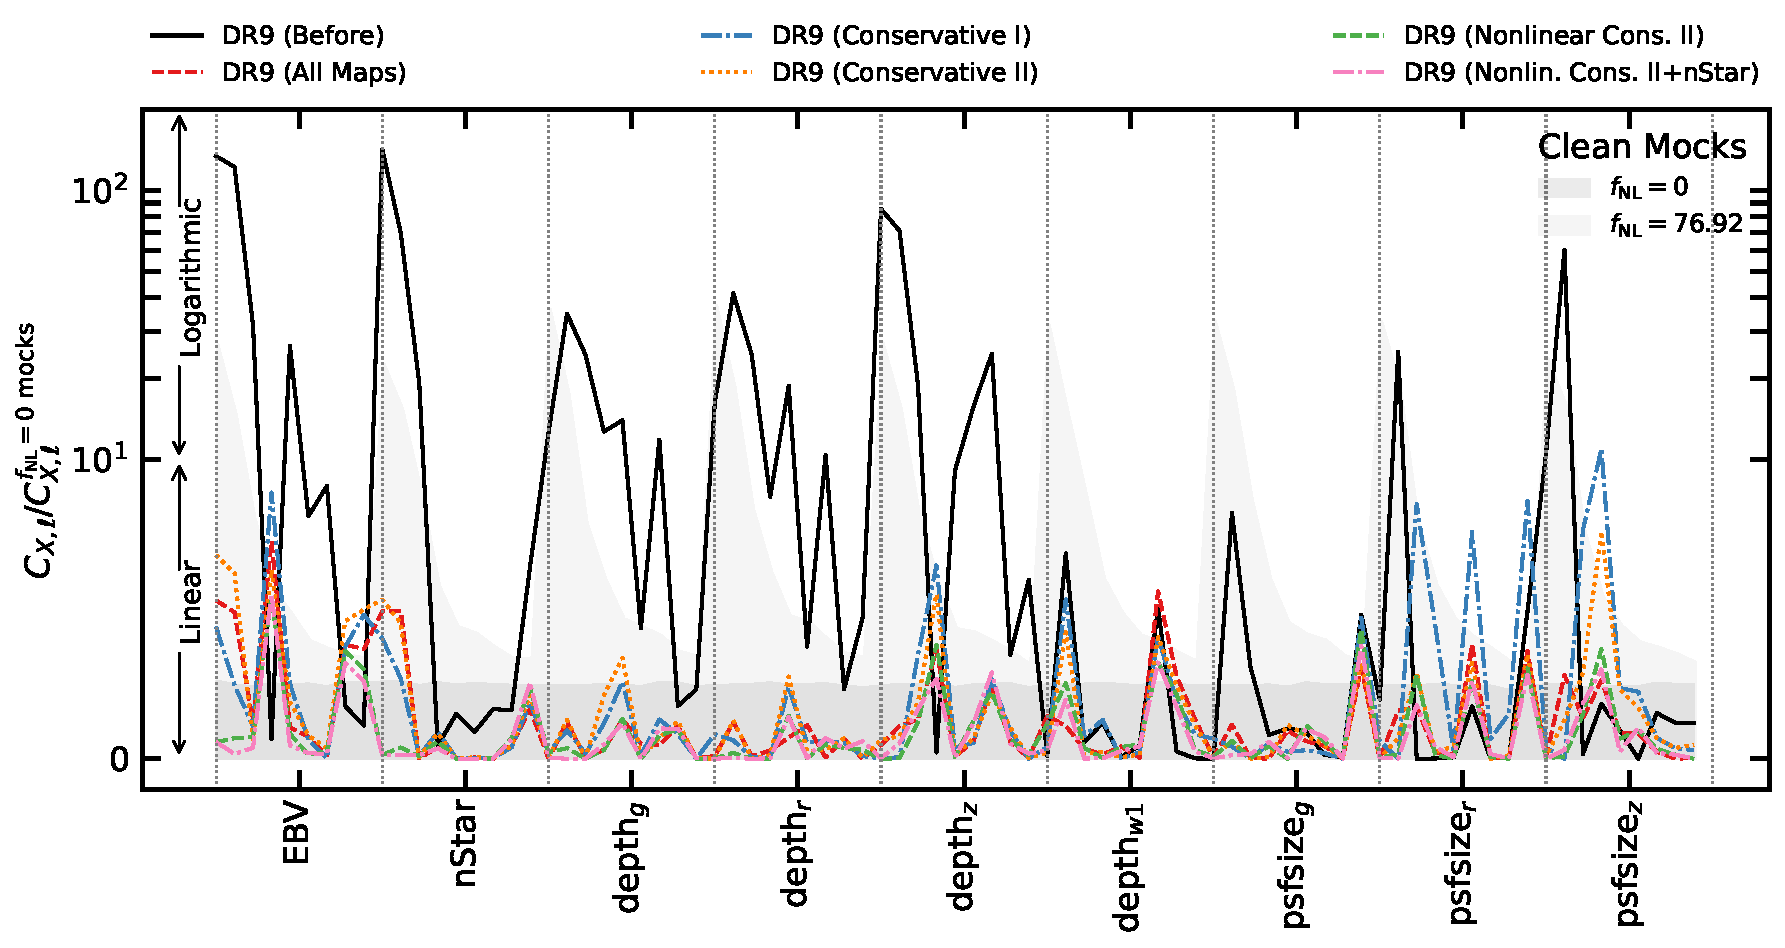
\includegraphics[width=0.95\textwidth]{clx_mocks.pdf}
\caption{Normalized cross power spectrum of mocks. Top: mean cross spectrum. Bottom: standard deviation.}\label{fig:clxmock}
\end{figure*}

\begin{figure}
\centering
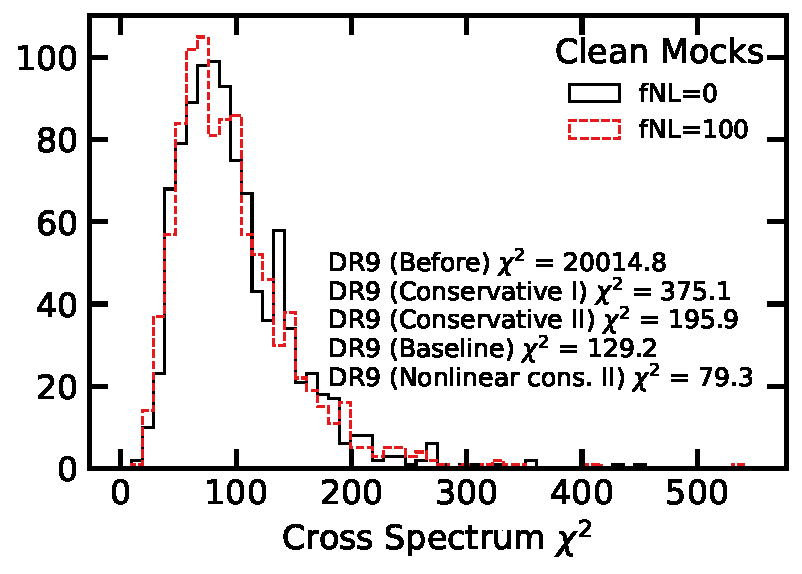
\includegraphics[width=0.45\textwidth]{chi2test.pdf}
\caption{Cross power spectrum $\chi^{2}$ diagnostic. The DR9 value is quoted and the histograms are constructed from 1000 realizations of mocks with $\fnl=0$ and $100$.}
\end{figure}


